% --------------------------------------------------------------
% This is all preamble stuff that you don't have to worry about.
% Head down to where it says "Start here"
% --------------------------------------------------------------

\documentclass[12pt]{article}

\usepackage[margin=1in]{geometry}
\usepackage{amsmath,amsthm,amssymb}
\usepackage{graphicx} %This allows to include eps figures
\usepackage{subcaption}
\usepackage[section]{placeins}
\usepackage{layout}
\usepackage{etoolbox}
\usepackage{mathabx}
\usepackage{animate}
\usepackage{array}
% This is to include code
\usepackage{listings}
\usepackage{xcolor}
\definecolor{dkgreen}{rgb}{0,0.6,0}
\definecolor{gray}{rgb}{0.5,0.5,0.5}
\definecolor{mauve}{rgb}{0.58,0,0.82}
\lstdefinestyle{Python}{
    language        = Python,
    basicstyle      = \ttfamily,
    keywordstyle    = \color{blue},
    keywordstyle    = [2] \color{teal}, % just to check that it works
    stringstyle     = \color{green},
    commentstyle    = \color{red}\ttfamily
}

\newenvironment{conditions}
  {\par\vspace{\abovedisplayskip}\noindent\begin{tabular}{>{$}l<{$} @{${}={}$} l}}
  {\end{tabular}\par\vspace{\belowdisplayskip}}

\newcommand{\N}{\mathbb{N}}
\newcommand{\Z}{\mathbb{Z}}

\newenvironment{theorem}[2][Theorem]{\begin{trivlist}
\item[\hskip \labelsep {\bfseries #1}\hskip \labelsep {\bfseries #2.}]}{\end{trivlist}}
\newenvironment{lemma}[2][Lemma]{\begin{trivlist}
\item[\hskip \labelsep {\bfseries #1}\hskip \labelsep {\bfseries #2.}]}{\end{trivlist}}
\newenvironment{exercise}[2][Exercise]{\begin{trivlist}
\item[\hskip \labelsep {\bfseries #1}\hskip \labelsep {\bfseries #2.}]}{\end{trivlist}}
\newenvironment{reflection}[2][Reflection]{\begin{trivlist}
\item[\hskip \labelsep {\bfseries #1}\hskip \labelsep {\bfseries #2.}]}{\end{trivlist}}
\newenvironment{proposition}[2][Proposition]{\begin{trivlist}
\item[\hskip \labelsep {\bfseries #1}\hskip \labelsep {\bfseries #2.}]}{\end{trivlist}}
\newenvironment{corollary}[2][Corollary]{\begin{trivlist}
\item[\hskip \labelsep {\bfseries #1}\hskip \labelsep {\bfseries #2.}]}{\end{trivlist}}



\begin{document}

% --------------------------------------------------------------
%                         Start here
% --------------------------------------------------------------

%\renewcommand{\qedsymbol}{\filledbox}

\title{Assignment 5}%replace X with the appropriate number
\author{Nalet Meinen and Pascal Wyss\\ %replace with your name
Finite Element Analysis I
}
\maketitle

\begin{figure}[!htb]
  \centering
  \vspace*{1cm}
  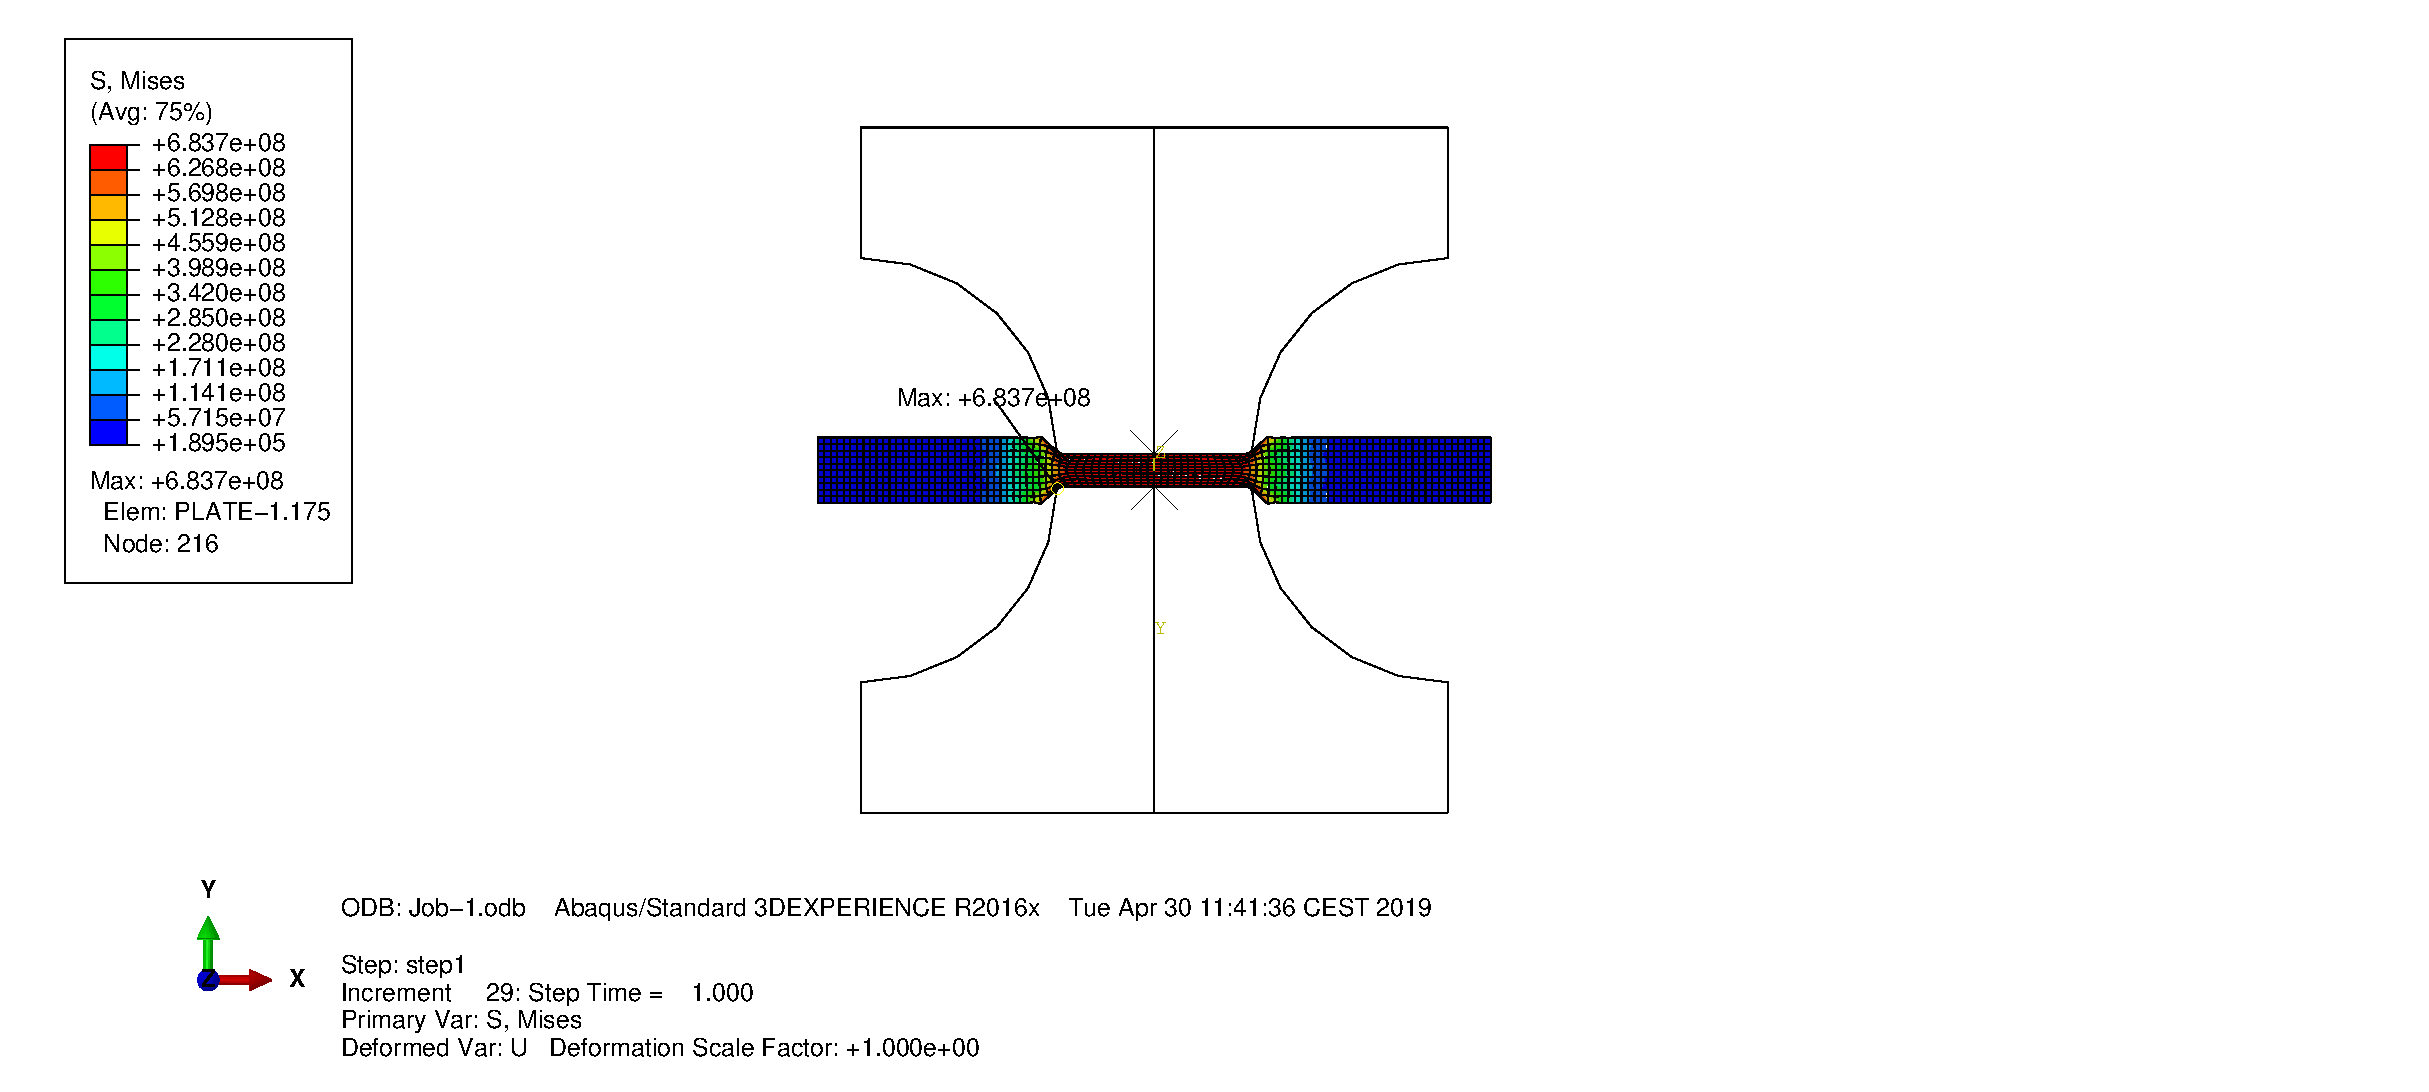
\includegraphics[trim={2cm 2cm 2cm 2cm},clip,width=1.0\linewidth]{pics/titelbild}
  \label{fig:0}
\end{figure}

\newpage

\section*{Abstract}
In this assignment, we examine the behavior of a metal plate under compression.
A rigid press, modeled as a 3D shell, squeezes the plate together.
By retrieving the force and displacement values over time, we can determine the plastic behavior 
of our specimen. In this assignment, we use the findings from the previous assignment 4 and 
instead of using a Lagrangian formulation we are using a Eulerian.


% \begin{figure}[!htb]
%   \centering
%   \animategraphics[autoplay,loop,width=0.8\linewidth,trim={1mm 1mm 1mm 1mm}]{4}{pics/out/ani-}{1}{62}
%   \caption{Animation of frequency on beam}
% \end{figure}

\tableofcontents
\pagebreak
\section{Introduction}
Like in the previous assignment 4, the plate is compressed from both sides. Symmetry is used to keeep
computation time low. 
Eulerian modeling can only be done on 3D models. As the previous model was in 2D, 
for this assignment we remodeled the parts in 3D. We use the same material coefficients
as in the previous assignment. 
Despite using 3D-modelling, our specimen consits of only one element in depth
with encastered front and back surfaces. The behaviour is therefore
2D-alike.

\begin{figure}[!htb]
  \centering
  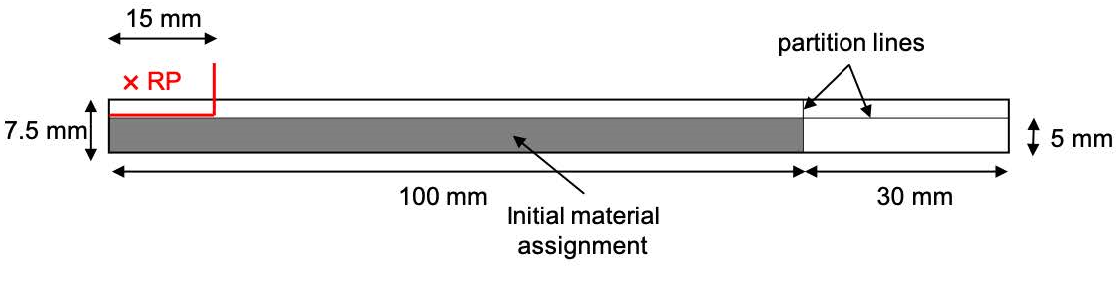
\includegraphics[width=1.0\linewidth]{pics/shematics}
  \caption{Model of the plate with Eulerian formulation}
  \label{fig:1}
\end{figure}

\noindent As shown in Figure \ref{fig:1}, the model of the plate has to be partitioned. 
We have to anticipate the final distribution of the material (white area), as Abaqus needs us to define the are/volume 
where the original material (shaded area) will be "flowing" during simulation. 
Again, only a quarter of the model has to be sketched due to symmetry.

\newpage
\section{Methods}

\subsection{Coupled Lagrangian-Eulerian Analysis in Abacus}

In this assignment we used eularian parts. The most obvious difference to the previous Lagrangian
simulations is the behaviour of the mesh during simulation. Whereas lagrangian meshes deform and compress 
with the part, eularian meshes stay intact. This, however, needs to be taken into account 
when meshing the part in the first place, as there has to be enough "meshed space" around the model,
where the material can flow into. This material flow is then measured to draw conclusions
about the material characteristics.

\begin{figure}[!htb]
  \centering
  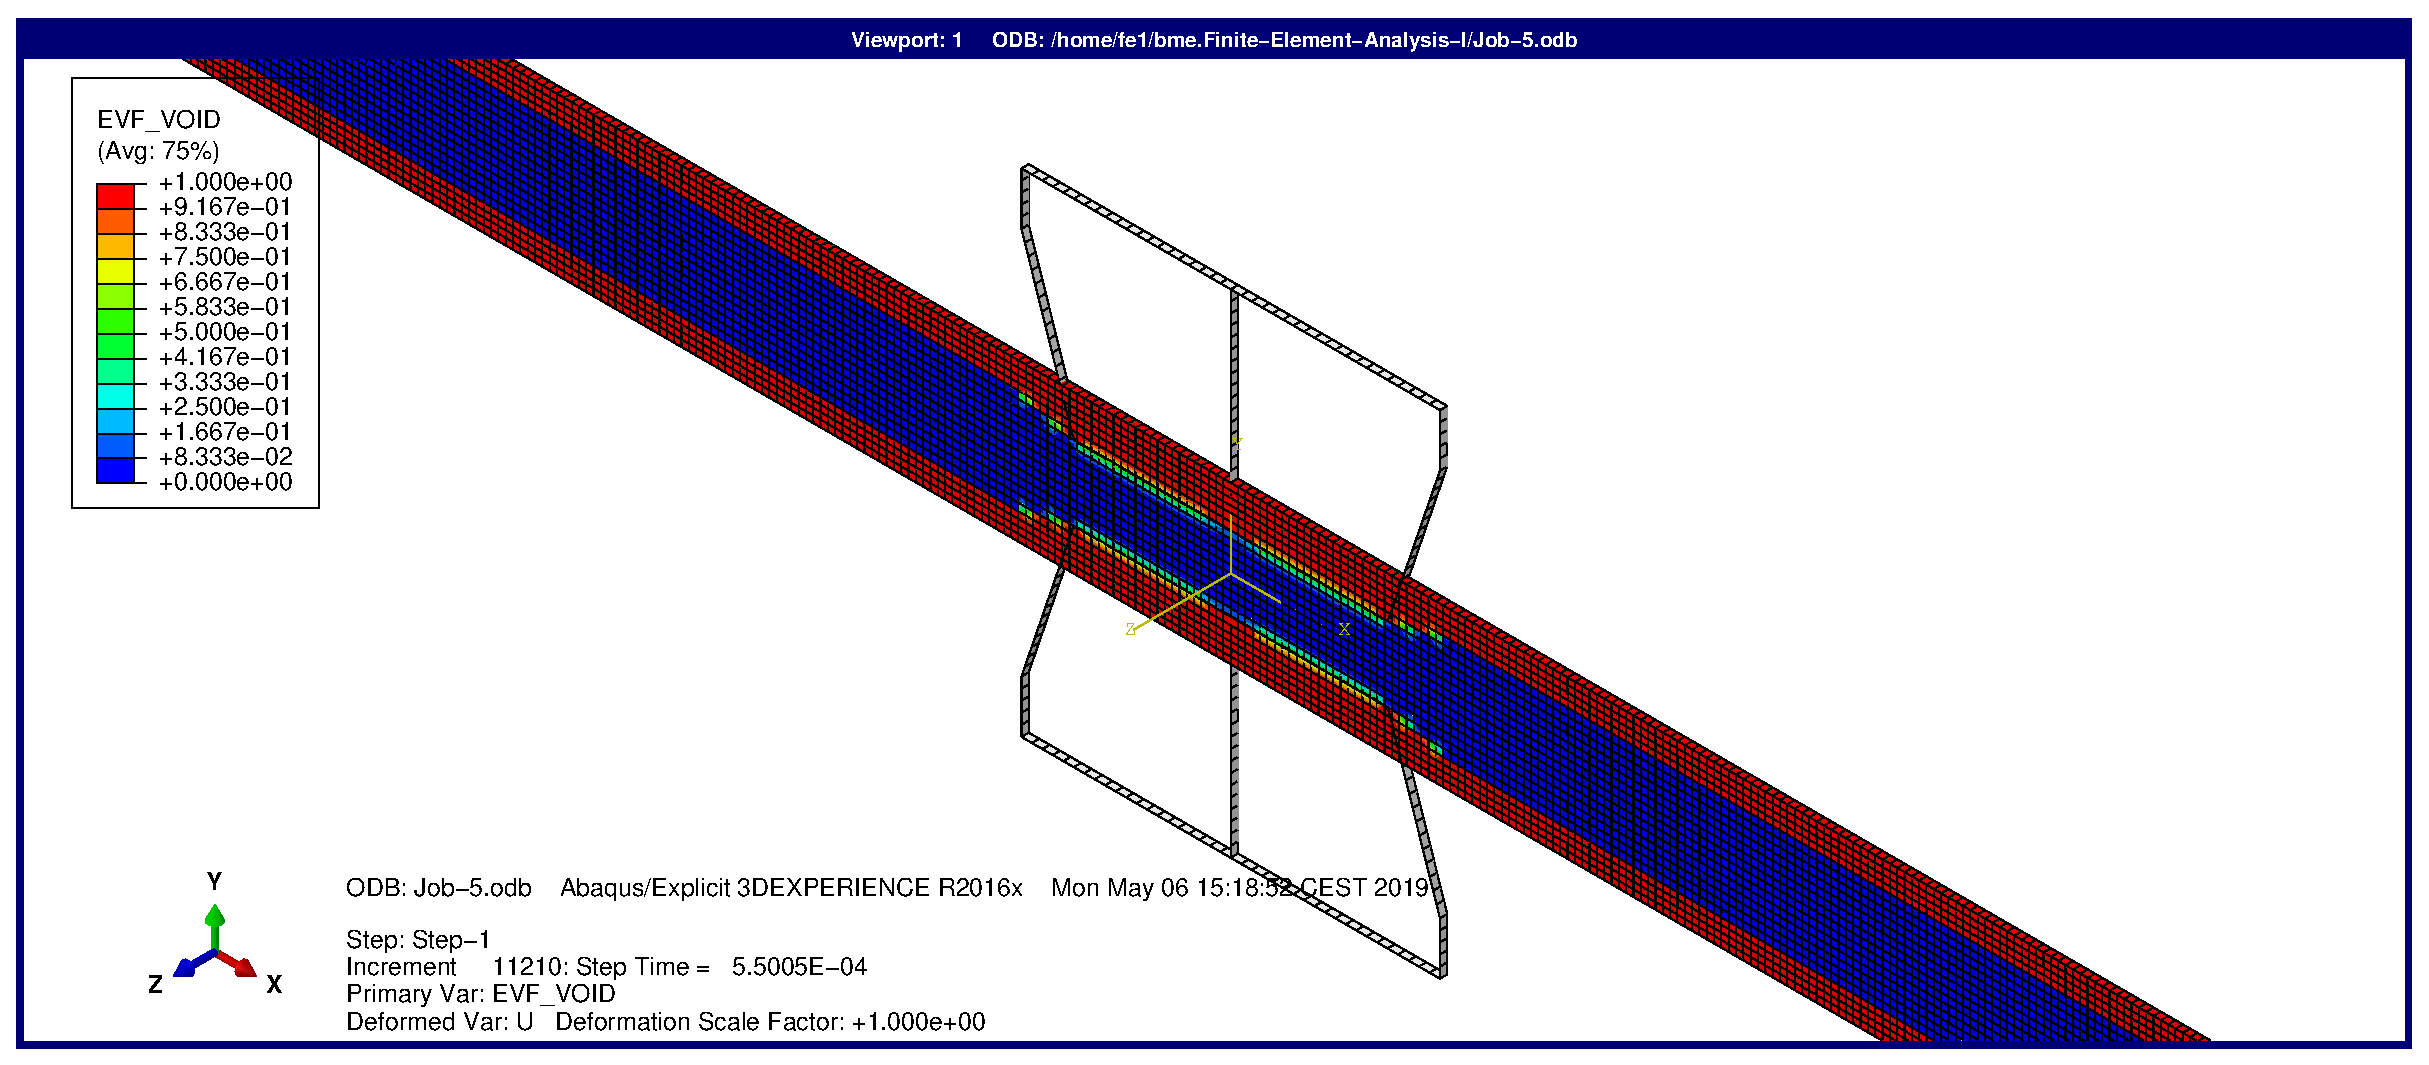
\includegraphics[width=0.9\linewidth]{pics/sexy3Dbild}
  \caption{mirrored 3D-model}
  \label{fig:2}
\end{figure}

\begin{figure}[!htb]
  \centering
  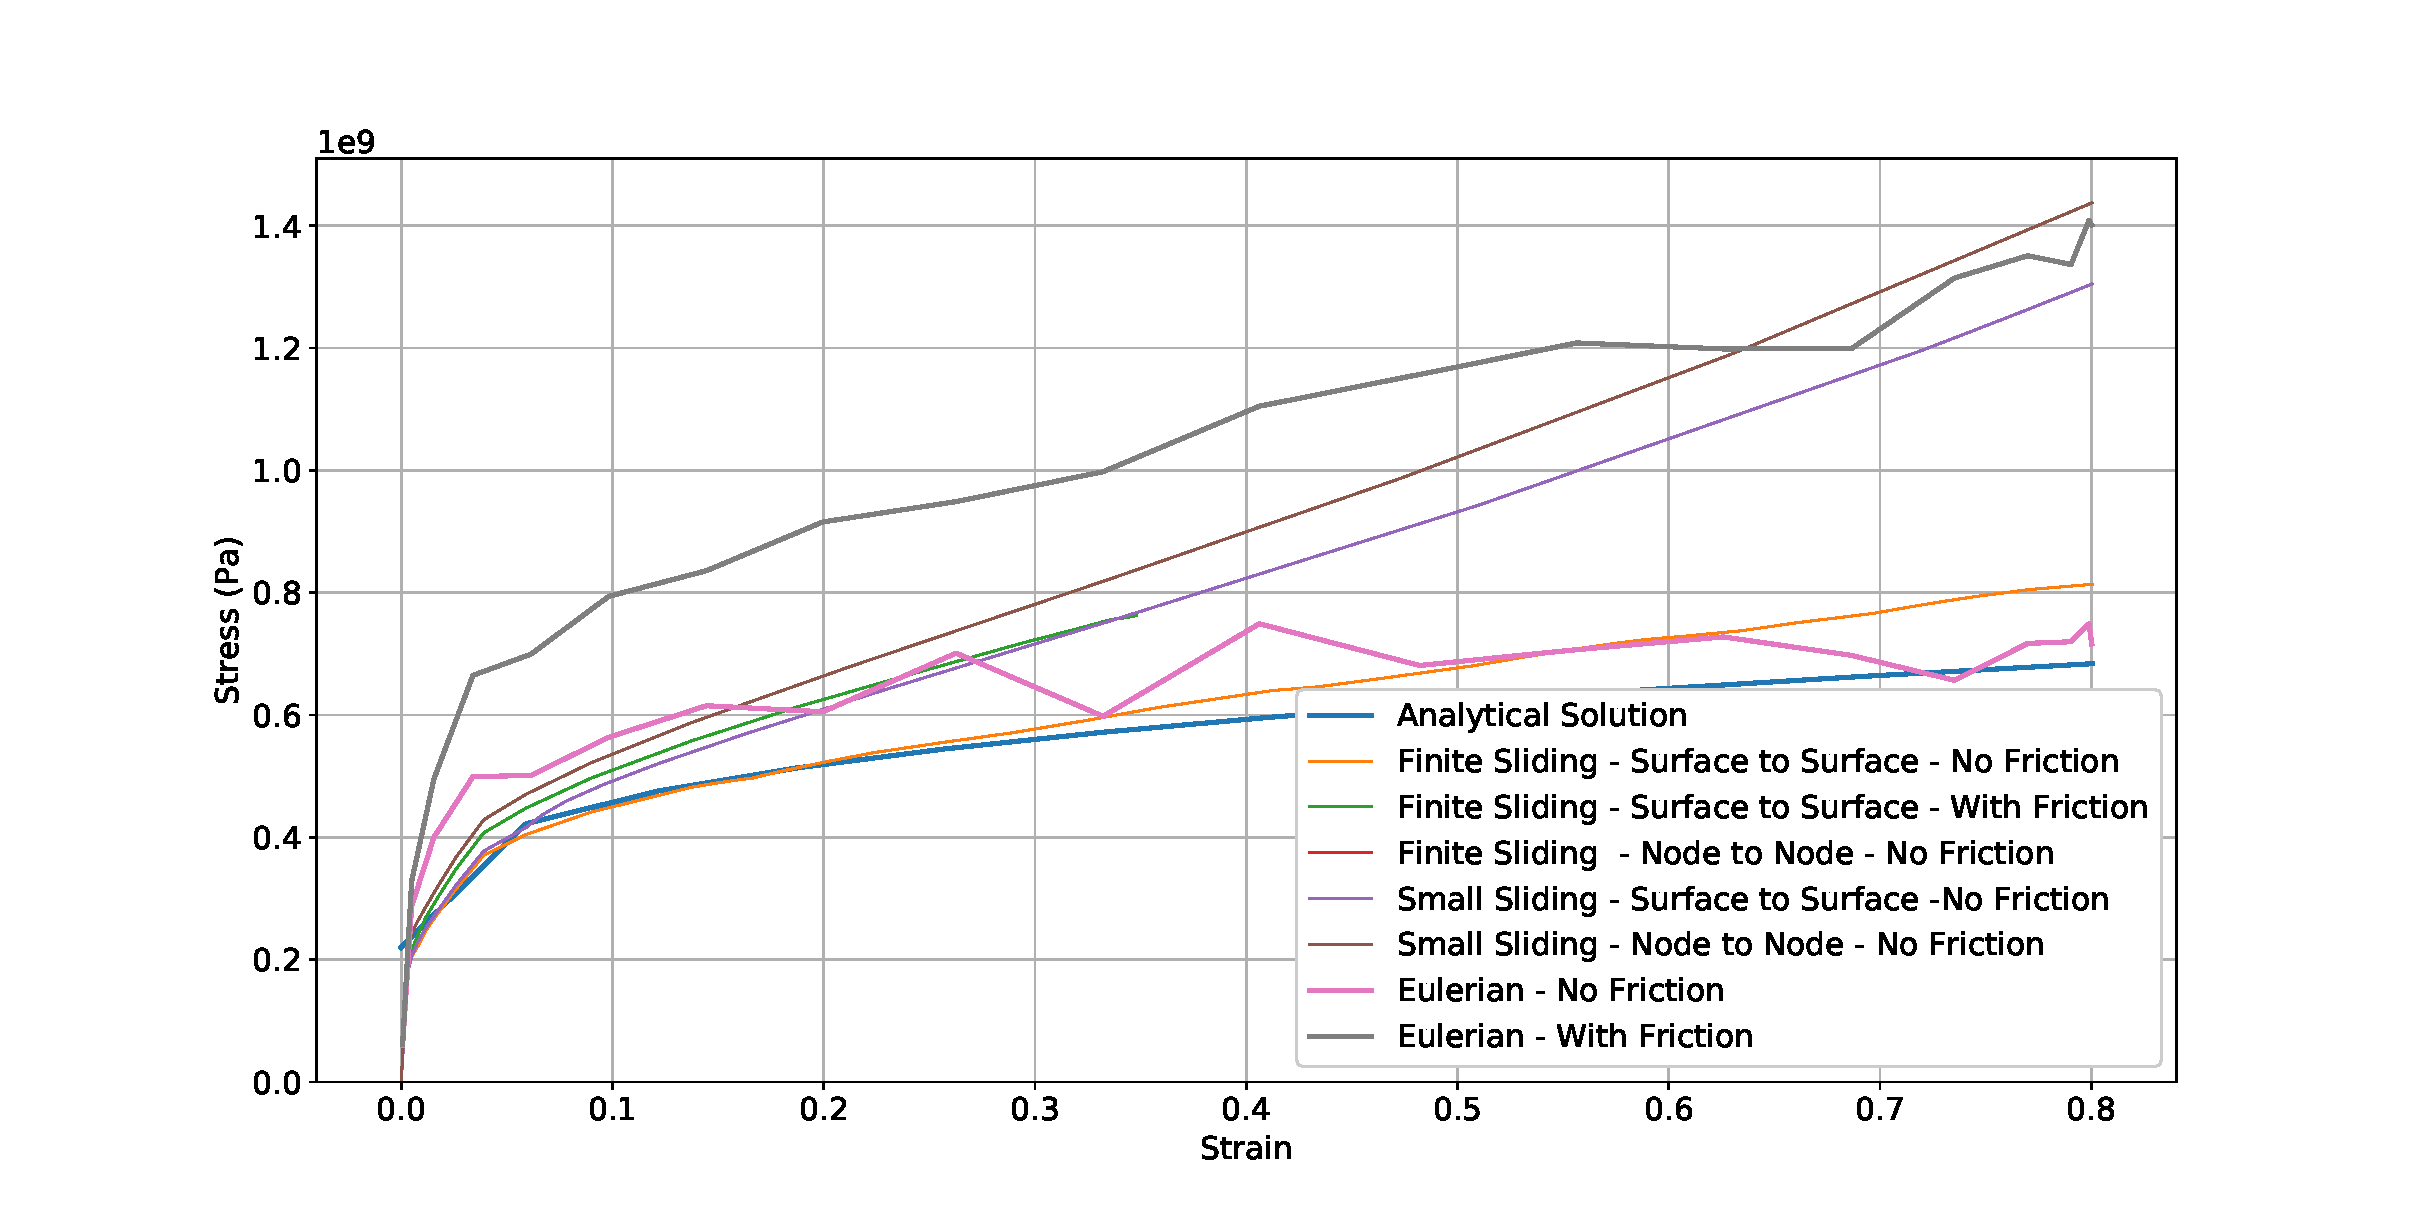
\includegraphics[width=0.9\linewidth]{pics/analytical_compared_euler}
  \caption{Result of the previous assignment amended with eulerian result}
  \label{fig:3}
\end{figure}


\pagebreak
\section{Results and Discussion}

The gained results from the eularian simulation are similar to the lagrangian results from the 
prvious assignment. Both simulations, with or without friction, lie in the region
of stress/strain ratio as in the previous assignment. We assume the lagrangian approach to be better or 
equal to eularian for small deformations. As soon as the deformations get larger, the lagrangian elements
will be deformed significantly, which may impact the accuracy. As the eularian mesh is independent
of the part, it stays in in its original shape.


\pagebreak
\begin{thebibliography}{9}
  \bibitem{latexcompanion} 
  Michel Goossens, Frank Mittelbach, and Alexander Samarin. 
  \textit{The \LaTeX\ Companion}. 
  Addison-Wesley, Reading, Massachusetts, 1993.
  \bibitem{assignment4} 
  Nalet Meinen, Pascal Wyss.
  \textit{FEM Assignment 4/2019}. 
\end{thebibliography}


\end{document}